\label{texfile:GWF}
Currently, every \mfus\ model must contain a \gwf\ domain, which may be reduced to a single layer of very low hydraulic conductivity in cases where \gwf\ flow and interaction with other model domains is to be neglected.

\subsection{Generating a Layered \gwf\ Domain}
A \mfus\ 3D groundwater flow (\gwf) domain can be generated from the template using this instruction:

\ins{generate layered gwf domain}
    {This subtask has instructions that are used to define:
     \begin{itemize}
        \item Element zone numbering scheme
        \item Top elevation of domain (e.g.\ ground surface)
        \item New mesh layers, vertical discretization (sublayering) and base elevation
    \end{itemize}

    An end instruction is required to stop the subtask e.g.:

    {\Large \sf end generate layered gwf domain}
    }

    {\em NOTE: The term layers used here should not be confused with the \mf\ term of the same name. A \mf\ layer is one cell thick, while a \mut\ layer can be one or more elements thick.}

The construction of the 3D \gwf\ finite-element mesh proceeds from top to bottom.  First, we define the top elevation, then add layers one at a time, defining the base elevation and vertical discretization of each new layer,  until we reach the base of the domain. By default, element zone numbering  corresponds with layer numbering.  Alternatively, if the template mesh is divided into horizontal patches with unique zone numbers, these can be assigned instead to the 3D GWF mesh using this instruction\footnote{The example \texttt{6\_Abdul\_Prism\_Cell} uses this option to define \swf\ domain zones.}:

\ins{Zone by template}
    {Causes \mut\ to assign the template mesh element zone number to the corresponding 3D \gwf\ element.  This results in zones that are vertical columns of elements from the top to the bottom of the \gwf\ domain.

    {\em This instruction should appear in the input file at the beginning of the \textsf{generate layered gwf domain} subtask before new layers are added.}
    }

\subsubsection{Defining the Top Elevation} \label{section:topelev}
To assign an elevation to the top layer of template nodes use this instruction:

\ins{top elevation}
    {This subtask defines the elevation (i.e. $z$-coordinate) of the top layer of nodes in the \gwf\ finite-element template mesh in one of these ways:
     \begin{itemize}
        \item By assigning a given elevation to all nodes
        \item By reading variable elevation data from a file
        \item By interpolating elevation data from a function $z(x)$ where the elevation $z$ varies by the nodal $x$ coordinate.
     \end{itemize}

    An end instruction is required to stop the subtask e.g.:

    {\Large \sf end top elevation}
    }

 The top elevation can be defined by one of these instructions: \label{'Page:TopElev'}

 \ins{elevation constant}
    {\squish
    \begin{enumerate}
    \item \rnum{Elev} [$L$]  The elevation \rnum{Elev} will be assigned to all top layer nodes.
    \end{enumerate}
    \squish
    }

 \ins{elevation from gb file}
    {\squish
    \begin{enumerate}
    \item \str{FName}  The elevation data in the \gb\ nodal property file \str{FName} will be assigned to the top layer nodes.
    \end{enumerate}
    \squish
    }

The \gb\ nodal property file uses a legacy binary file format. You can develop your own ascii input files and read them using this instruction:

 \ins{elevation from list file}
    {\squish
    \begin{enumerate}
    \item \str{FName}  The elevation data in the ascii file \str{FName} will be assigned to the top layer nodes.
    \end{enumerate}
    \squish
    }

Part of a sample list file\footnote{The example \texttt{6\_Abdul\_MODHMS} uses an ascii file input to define nodal elevations.} is shown here:
    \begin{verbatim}
    Kriged cell top elevation for layer 1
     4.414571762E+000
     4.415914536E+000
     ...
     4.415914536E+000
     \end{verbatim}
     \squish
Some key features of this example are:
\begin{itemize}
  \item The first line of the file is discarded, and in this case contains a string describing the data.
  \item You must supply a value for each node in the template finite-element mesh.
  \item The data is read in free format so there can be more than one value entered per line.
  \item Only the start and end of the file are shown here, with the string '\texttt{...}' replacing the middle portion.
\end{itemize}

To define the top elevation as a function of $x$ (usually used for 2D cross-sectional models) use this instruction:

 \ins{elevation from xz pairs}
    {
    \squish
    \begin{enumerate}
    \item \rnum{x(1)} [$L$], \rnum{z(1)} [$L$]  First $x, z$ coordinate pair.
    \item \textbf{...} \\
     \hspace*{-.27in}\rule{0.in}{.24in}  n. \rnum{x(n)} [$L$], \rnum{z(n)} [$L$]  nth $x, z$ coordinate pair.
    \end{enumerate}

     An elevation is calculated for each chosen cell, based on it's $x$-coordinate location, by interpolating an elevation from the given list of  $xz$-coordinate pairs.

    An end instruction is required to stop the subtask e.g.:

    {\Large \sf end elevation from xz pairs}
    }

Here is an example showing the use of this instruction\footnote{The example \texttt{1\_VSF\_Hillslope} uses the \textsf{elevation from xz pairs} instruction to define the top elevation of the cross-sectional domain.}:
    \begin{verbatim}
    elevation from xz pairs
           0.0,   0.0
        1000.0, 100.0
    end elevation from xz pairs
     \end{verbatim}
     \squish
Some key features of this example are:
\begin{itemize}
  \item The two given $xz$ pairs define a line that slopes from $z=0$ at $x=0$ to $z=100.0$ at $x=1000$.  You may supply as many pairs as needed to define the top of your cross-section.
  \item $x$ coordinates must increase continuously from the top of the list to the bottom.
  \item the $x$-range of the supplied pairs should cover the entire $x$-range of the template mesh.
  \item For each node in the template mesh, the $x$ coordinate is used to interpolate an elevation (i.e. $z$ value) using the appropriate $xz$ pair.
\end{itemize}

To define the top elevation as a function of $x$ and $y$ (for 3D models) use this instruction:

 \ins{elevation from bilinear function in xy}
    {
    \squish
    \begin{enumerate}
    \item \rnum{xfrom} [$L$], \rnum{xto} [$L$], \rnum{yfrom} [$L$], \rnum{yto} [$L$]  $x$ and $y$ coordinates ranges.
    \item \rnum{a1}, \rnum{a2}, \rnum{a3}, \rnum{a4}, \rnum{a5}  Constants for the bilinear function.
    \end{enumerate}
    For nodes falling within the given $x$ and $y$ range, the z-coordinate is
    computed according to the following function:
    \begin{displaymath}
        z = \textbf{a1} + \textbf{a2} (x-\textbf{xfrom}) + \textbf{a3}*(x-\textbf{xfrom})^2
            + \textbf{a4}(y-\textbf{yfrom}) + \textbf{a5}(y-\textbf{yfrom})^2
    \end{displaymath}
    }

Here is an example showing the use of this instruction\footnote{The example \texttt{8\_V\_catchment} uses the \textsf{elevation from bilinear function in xy} instruction to define the top elevation of a portion of the 3D domain.}:
    \begin{verbatim}
        elevation from bilinear function in xy
        0.0 800.0 0.0 1000.0
        41.0 -0.05 0.0 0.02 0.0

        elevation from bilinear function in xy
        800.01 819.99 0.0 1000.0
        1.0 0.0 0.0 0.02 0.0

        elevation from bilinear function in xy
        820.0  1620.01 0.0 1000.0
        1.0 0.05 0.0 0.02 0.0
     \end{verbatim}
     \squish
Some key features of this example are:
\begin{itemize}
  \item Three sets of \textsf{elevation from bilinear function in xy} instructions define a tilted catchment with 3 sections.
  \item If a node in the template mesh falls within a bilinear function $xy$-range, then that function is used to interpolate an elevation (i.e. $z$ value) for the node.
  \item The $xy$-ranges supplied should cover the entire top of the template mesh.
\end{itemize}


\pagebreak
\subsubsection{Adding Layers} \index{\gwf\ Domain ! layering}
A \mfus\ model must contain at least 1 layer, and each layer is defined using this instruction:     {\index{Grid generation ! \gwf\ Domain ! New layer}

\ins{new layer}
    {This subtask adds a new layer to the \gwf\ domain by defining the layer:
     \begin{itemize}
       \item Base elevation
       \item Vertical discretization
     \end{itemize}

    An end instruction is required to stop the subtask e.g.:

    {\Large \sf end new layer}
    }

The base elevation is defined using the elevation instructions  described on page~\pageref{'Page:TopElev'} that are given for the \textsf{top elevation} instruction.

By default, \mut\ will stop and issue a warning message if the computed layer base elevation is greater than or equal to the current layer top elevation.  This instruction forces the base to be below the top by a set amount:

\ins{Minimum layer thickness}
    {\squish
    \begin{enumerate}
    \item \rnum{MinThick}[L]  Minimum thickness value.
    \end{enumerate}
    This instruction causes \mut\ to enforce a minimum thickness constraint for the current layer. At nodes where the computed layer base elevation is greater than or equal to the current top elevation, \rnum{MinThick} will
    be subtracted from the current top elevation to get the base elevation.
    }


By default, a new layer will be assigned the name '\texttt{Layer {\em n}}' where {\em n} is the current layer number.  If you want to assign your own layer name use this instruction:

\ins{Layer name}
    {
    \squish
    \begin{enumerate}
    \item \str{LayerName} Layer name.
    \end{enumerate}
    \squish
    }

%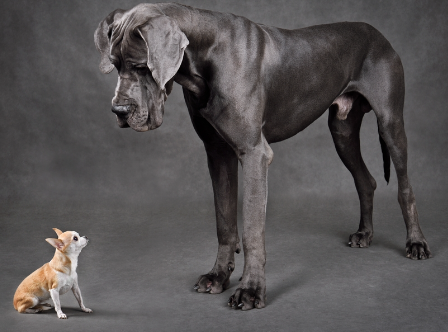
\includegraphics[width=.15\textwidth]{ModelDevelopment} \textit{These names are not currently used in Tecplot output but could/should? be used to create the customlables for zone naming.}

By default, a new layer will not be subdivided vertically unless one the following two instructions is issued.
The first creates a uniform subdivision:

\ins{Uniform sublayering}
    {\squish
    \begin{enumerate}
    \item \inum{nsublayer} Number of sublayers.
    \end{enumerate}
    This instruction divides the layer vertically into \inum{nsublayer}
    elements, which will each have the same element height, equal to the top elevation
    minus the current base elevation divided by \inum{nsublayer}.
    }

This instruction creates a non-uniform subdivision\footnote{The example \texttt{6\_Abdul\_MODHMS} uses the \textsf{Proportional sublayering}  instruction to match the cell top elevations of the original {\sc MODHMS} mesh.}:

\ins{Proportional sublayering}
    {\squish
    \begin{enumerate}
        \item \inum{nSublayer}  Number of proportional sublayers.
        \item \rnum{SubThick(i)}, i=1,\inum{nSublayer} Proportional thicknesses in order from top to bottom.
    \end{enumerate}
    This instruction can be used if you want to refine the \gwf\ domain mesh vertically,
    for example, in the active zone near the \swf\ domain at ground surface.

    It is important to understand that the variable \rnum{SubThick} is not
    a true thickness, but is instead a dimensionless relative thickness, which is used along
    with the layer thickness to determine the element heights in the current
    column.
}

    For example, these instructions:
    \texttt{
            \begin{tabbing}
            AAA\=AAA\=AAA   \kill
                \>Proportional sublayering   \\
                \>   \> 3                     \\
                \>   \> 0.1           \\
                \>   \>1.0            \\
                \>   \>  10.0       \\
                \> end       \\
            \end{tabbing}
    }
    \squish
would subdivide the current layer vertically into three elements, between
    the current base and top elevation, with the middle element being ten times as thick as the top element, and 1/10th as thick as the bottom element.

This instruction can be used to create a basal layer surface a given distance below, and parallel to, it's top surface:

\ins{Offset base}
    {\squish
    \begin{enumerate}
        \item \rnum{Offset} [$L$] Height of offset.
    \end{enumerate}
    This instruction causes the elevation of layer base to be offset below the  top by the  value \rnum{Offset}.
}

\pagebreak
For example, these instructions:
\begin{verbatim}
        top elevation
            elevation from list file
            elev.list
        end top elevation

        new layer
            uniform sublayering
            3

            elevation from list file
            elev.list

            offset base
            -1.0

        end new layer

    end generate layered gwf domain
\end{verbatim}
 create a layer with a top elevation 1 length unit (e.g.\ 1 meter) below the elevation defined in the raster file \texttt{elev.list}:

%
\includegraphics[width=.15\textwidth]{UnderConstruction} \textit{Need to check sign on \textsf{offset base} input}

\subsubsection{Cell Connection Properties}
\label{section:GWFCellConnections}
\index{\gwf\ Domain ! cell connection properties}

Currently, \mut\ defines lateral connections between neighbouring cells (i.e. that share a common side) in the template 2D finite element mesh, and vertical connections between neighbouring cells (i.e. that share a common face) in the stacked 3D \gwf\ finite-element mesh.

The \gwf-\gwf\ cell connection length (distance from cell to cell) and area (cross-sectional area perpendicular to the direction of flow) vary on a cell-by-cell basis, and depend on control volume approach (mesh- or node-centred) and element shape (triangle or rectangle).

Consider the mesh-centred case, where cell control volumes are defined at the triangular element centroid:

        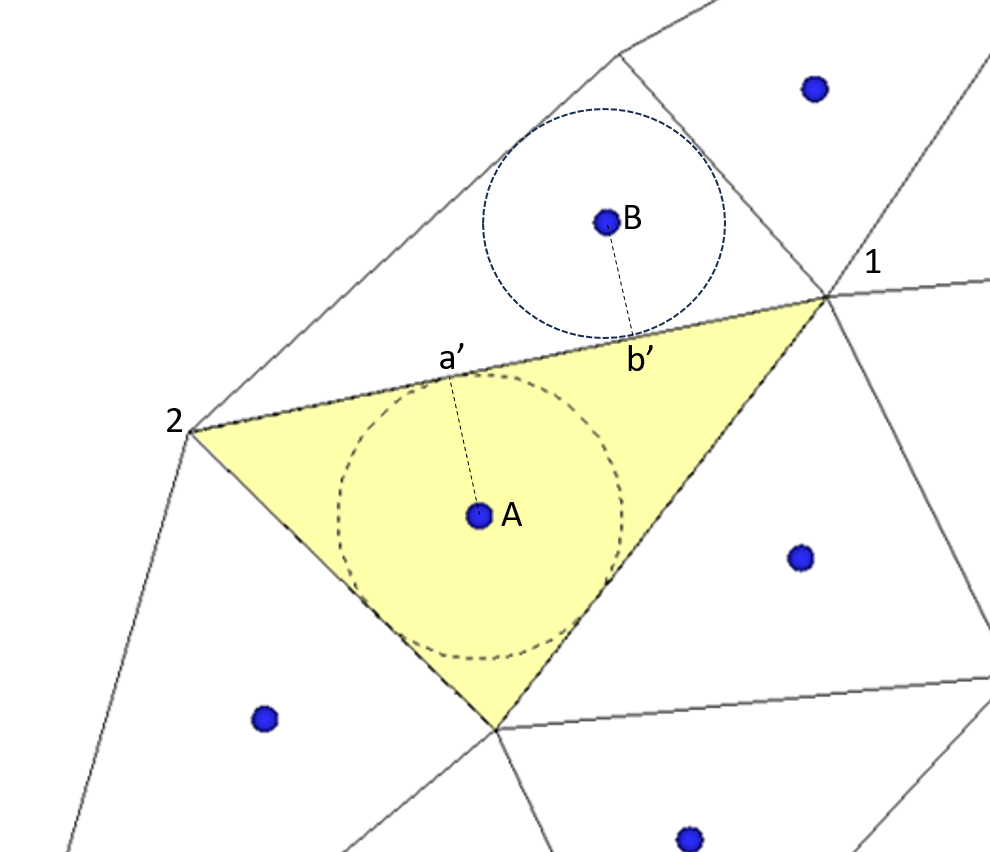
\includegraphics[width=0.6\textwidth]{3_8b_MeshCentredCellConnection}

The yellow triangle shows the footprint of a \mfus\ cell.

Cell B is a lateral neighbour of cell A and shares side 1-2.  The lateral connection length between A and B is the sum of the lengths of the inner circle radii for each cell: A-a' + B-b'.  The lateral connection area is the product of the length of the shared side 1-2 and the cell thickness.

In the vertical direction, cells above and below cell A are its neighbours.  The vertical connection length is the sum of the two half-cell thicknesses. The vertical connection area equals the area of the template mesh element (yellow triangle).

Here is the node-centred case, where cell control volumes are defined at the triangular element node:

        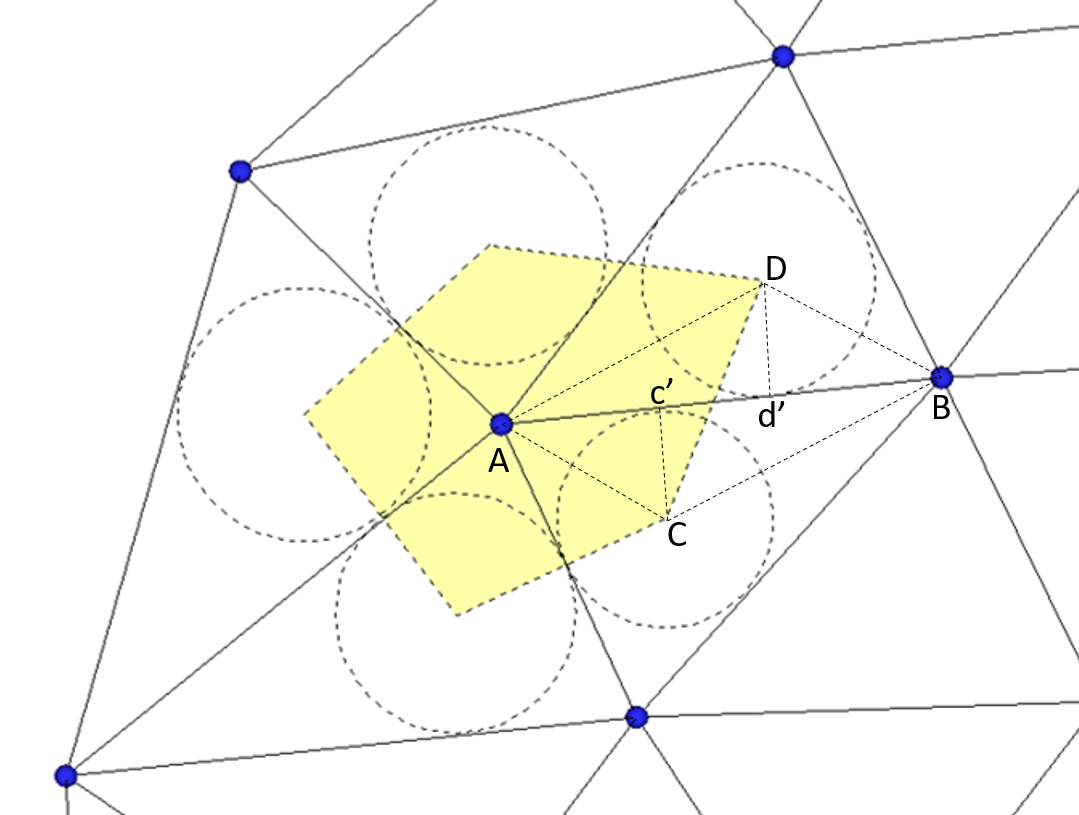
\includegraphics[width=0.6\textwidth]{3_8b_NodeCentredCellConnection}

The yellow polygon shows the footprint of a \mfus\ cell.

Cell B is a lateral neighbour of cell A.  The lateral connection length between A and B is the distance from node A to node B. The lateral connection area is defined by the sum of the inner circle radii for each neighbouring triangle: C-c' + D-d' and the cell thickness.

In the vertical direction, cells above and below cell A are its neighbours.  The vertical connection length is the sum of the two half-cell thicknesses. The vertical connection area is the area of the polygon formed by joining the inner circle centres of the template mesh elements common to cell A (yellow polygon).

Cell connection data are defined in a similar fashion for model domains that are generated from a rectangular element template mesh.  In this case, element side lengths are used to define connection lengths and areas instead of inner circle radii.


\subsubsection{Material Properties}  \index{\gwf\ Domain ! material properties} \label{section:matprops}

\gwf\ domain material properties may vary on a cell-by-cell  basis.  \mut\ has instructions for selecting subsets of cells. A cell is selected when a true/false attribute (referred to as  the cells \textsf{Chosen} attribute) is set to true. Selected cells can be assigned material property values.  This instruction selects all cells in the {\em active} model domain:

\ins{choose all cells}
    {Select all cells in the active model domain.
     }

  This is an example of what we refer to as a {\em generic} instruction, which means it will be applied to the currently active model domain: \gwf, \swf\ or \cln.  To choose all cells in the \gwf\ domain, we first need to activate it using this instruction:

\ins{active domain}
    {
        \squish
        \begin{enumerate}
        \item \str{Domain}  The name of the domain to be activated: \gwf, \swf\ or \cln\
        \end{enumerate}
        This instruction activates the given domain named in  \str{Domain} so that it will be used with generic instructions such as \textsf{choose all cells}.
    }

So to activate the \gwf\ domain, we would insert these instructions in the input file:
\begin{verbatim}
    active domain
    gwf
\end{verbatim}

These instructions can now be used to choose \gwf\ cells in various ways\label{page:cellSelect}:

\ins{choose cell at xyz}
    {
        \squish
        \begin{enumerate}
        \item \rnum{x1} [$L$], \rnum{y1} [$L$], \rnum{z1} [$L$]  An $xyz$ coordinate triplet.
        \end{enumerate}
        The cell closest to the given $xyz$ coordinate triplet will be chosen.
    }

\ins{choose cells by layer}
    {
        \squish
        \begin{enumerate}
        \item \inum{Layer}  The number of the layer to be chosen.
        \end{enumerate}
        The cells in Modflow layer number \inum{Layer} will be chosen.  Remember that Modflow layers are one cell high and are numbered from the top to the bottom of the model domain.\footnote{ See the example \texttt{1\_VSF\_Column} which uses the previous two instructions to define a constant head at  the base  and a recharge boundary condition at the top of the 1D column.}
    }

\ins{choose cells from file}
    {
        \squish
        \begin{enumerate}
        \item \str{FName}  The file \str{FName} containing a list of cell numbers.
        \end{enumerate}
        The cells listed in the file \str{FName} will be chosen.\footnote{ See the example \texttt{1\_Abdul\_MODHMS} which uses this instruction to assign some cells as inactive.}
    }

\ins{choose cells from gb elements}
    {
        \squish
        \begin{enumerate}
        \item \str{FName}  The \gb\ chosen element file \str{FName} containing information concerning the status, chosen or not chosen, of each element in the \gb\ model domain.
        \end{enumerate}
          If an element is flagged as chosen in the \gb\ model domain then the corresponding cell will be chosen in the \mfus\ model domain.\footnote{ See the  example \texttt{1\_Abdul\_Prism\_Cell} which uses this instruction to assign some cells as inactive.}
    }

\ins{choose cells from gb nodes}
    {
        \squish
        \begin{enumerate}
        \item \str{FName}  The \gb\ chosen node file \str{FName} containing information concerning the status, chosen or not chosen, of each node in the \gb\ model domain.
        \end{enumerate}
          If a node is flagged as chosen in the \gb\ model domain then the corresponding cell will be chosen in the \mfus\ model domain.\footnote{ See the  example \texttt{1\_Abdul\_Prism\_Cell\_nc} which uses this instruction to assign some cells as inactive.}
    }

The previous two instructions are used to choose cells for the mesh-centered and node-centered approaches respectively.

\pagebreak
Cell selection instructions are cumulative.  For example, you can modify the current selection by repeating instructions like  \textsf{choose cell at xyz} or \textsf{choose cells by layer} with different inputs and then assign properties to the current selection.  This instruction clears the selection before beginning new cell selection(s):

\ins{clear chosen cells}
    {Clears the current cell selection.
     }

It is good practice to clear the selection before starting a new selection. \mut\ echoes the results of the selection instructions to the screen and \texttt{.eco} file as shown in this example:
\begin{verbatim}
    clear chosen cells
    	GWF Cells chosen:          0

    choose all cells
    	GWF Cells chosen:      39765
\end{verbatim}
If a cell selection instruction has unexpected results it is good practice to check the \texttt{.eco} file for these outputs.

The recommended way to assign domain material properties is through the use of a lookup table.
\label{page:LookupTable}
\phantomsection\label{page:LookupTable}
Lookup tables are provided for each domain in the \bin\ directory, as outlined on page~\pageref{page:userbin}. In this case, the file \texttt{GWF.csv} contains the lookup table for the \gwf\ domain.

In order for \mut\ to access the lookup table, you first need to provide a link to this file using the instruction:

\ins{gwf materials database}
    {
        \squish
        \begin{enumerate}
        \item \str{FName}  \gwf\ material properties lookup table file name.
        \end{enumerate}
          \mut\ uses the file \str{FName} to look up \gwf\ material properties.
    }

In the case of the \gwf\ domain, the instructions:
\begin{verbatim}
    gwf materials database
    GWF.csv
\end{verbatim}
would be used to link to the lookup table.

You can now assign a set of \gwf\ material properties to the current cell selection using this instruction:

\ins{chosen cells use gwf material number}
    {
        \squish
        \begin{enumerate}
        \item \inum{MaterialID}  \gwf\ material ID number.
        \end{enumerate}
          The unique set of \gwf\ material properties with ID number \inum{MaterialID} is retrieved from the lookup table and assigned to the chosen cells.
    }

The example \texttt{1\_VSF\_Column} uses the following instructions to assign units of length and time for the \mfus\ model and the properties of the material with ID number 1 as shown here:
\begin{verbatim}
    build modflow usg
        units of length
        centimeters

        units of time
        days

        ... etc

        gwf materials database
        GWF.csv

        active domain
        gwf
           choose all cells

            chosen cells use gwf material number
            1
\end{verbatim}
The line \texttt{'...\ etc'} indicates a section of the input file that did not need to be shown for the purposes of this example.

The first few lines of the \texttt{GWF.csv} file are shown here:

    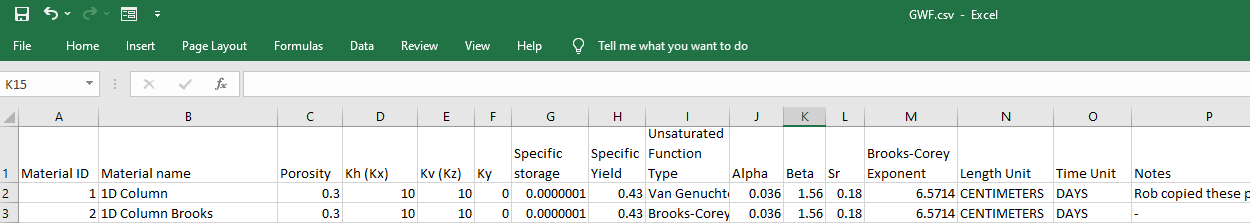
\includegraphics[width=0.95\textwidth]{3_11_GWFcsv}

Some key features to note are:
\begin{itemize}
    \item CSV files can be loaded and examined using \excel.
    \item The first line is a header with contains field (i.e. column) names.
    \item The first column contains the material ID number, followed by the material parameters (one per column), unit definitions and notes.
    \item Material 1 defines length units of centimeters and time units of days.  If these are the same as the defined \mfus\ unit system then no unit conversion is required, otherwise parameter values will be converted into the defined \mfus\ unit system according to their dimensionality.
\end{itemize}

Shown below is the output echoed to the screen and \texttt{\_buildo.eco} file for the example \texttt{1\_VSF\_Column}: \begin{verbatim}
    gwf materials database
        Materials file C:\MUT\MUT_Examples-main\_MUT_USERBIN\GWF.csv

    active domain
        gwf

    choose all cells
        GWF Cells chosen:        100

    chosen cells use gwf material number
        Assigning all chosen GWF cells properties of material     1, 1D Column
        Kh_Kx:                  10.000         CENTIMETERS   DAYS^(-1)
        Kv_Kz:                  10.000         CENTIMETERS   DAYS^(-1)
        Specific Storage:      1.00000E-07     CENTIMETERS^(-1)
        Specific Yield:        0.43000         DIMENSIONLESS
        Alpha:                 3.60000E-02     CENTIMETERS^(-1)
        Beta:                   1.5600         DIMENSIONLESS
        Sr:                    0.18140         DIMENSIONLESS
        Unsaturated Function Type:   Van Genuchten

\end{verbatim}
Some key features to note are:
\begin{itemize}
    \item The location and name of the materials database file used are shown.
    \item The material name (\texttt{1D Column}) associated with material ID number 1 is shown.
    \item The units defined in the database for each property are given. For example, property  \texttt{Kh\_Kx} has units of \verb+CENTIMETERS DAYS^(-1)+, where the string \verb+^(-1)+ means 'raised to the power of minus 1', giving units of \verb+CENTIMETERS/DAYS+.
\end{itemize}

Editing the \texttt{csv} files directly is not recommended. To modify existing or define new database files, please refer to the guidelines given in Appendix~\ref{Appendix:ExcelUseage}.

The following section describes instructions used to assign values to individual materials properties for the current cell selection.  When using these instruction, {\em you must be careful to supply the values in the unit system defined for the model}. This first instruction is used to define the horizontal hydraulic conductivity, \texttt{Kh}:

\ins{gwf kh}
    {
        \squish
        \begin{enumerate}
        \item \rnum{Kh} [$L$   $T^{-1}$]  Horizontal hydraulic conductivity.
        \end{enumerate}
          A horizontal hydraulic conductivity of \rnum{Kh} is assigned to the chosen cells.
    }

As a reminder to be aware of units, \mut\ will echo the assumed units to the screen and \texttt{o.eco} file e.g.:
\begin{verbatim}
    gwf kh
    	Assigning all chosen GWF cells a Kh of 0.10000E-04 CENTIMETERS DAYS^(-1)
\end{verbatim}

\ins{gwf kv}
    {
        \squish
        \begin{enumerate}
        \item \rnum{Kv} [$L$   $T^{-1}$]  Vertical hydraulic conductivity.
        \end{enumerate}
          A vertical hydraulic conductivity of \rnum{Kv} is assigned to the chosen cells.
    }

\ins{gwf ss}
    {
        \squish
        \begin{enumerate}
        \item \rnum{Ss} [$L^{-1}$]  Specific storage.
        \end{enumerate}
          A specific storage of \rnum{Ss} is assigned to the chosen cells.
    }

\ins{gwf sy}
    {
        \squish
        \begin{enumerate}
        \item \rnum{Sy}  Specific yield.
        \end{enumerate}
          A specific yield of  \rnum{Sy} is assigned to the chosen cells.
    }

\ins{gwf alpha}
    {
        \squish
        \begin{enumerate}
        \item \rnum{Alpha} [$L^{-1}$]  Van Genuchten/Brooks-Corey Alpha.
        \end{enumerate}
          A Van Genuchten/Brooks-Corey Alpha of \rnum{Alpha} is assigned to the chosen cells.
    }

\ins{gwf beta}
    {
        \squish
        \begin{enumerate}
        \item \rnum{Beta}  Van Genuchten/Brooks-Corey Beta.
        \end{enumerate}
          A Van Genuchten/Brooks-Corey Beta of \rnum{Beta} is assigned to the chosen cells.
    }

\ins{gwf sr}
    {
        \squish
        \begin{enumerate}
        \item \rnum{Sr}  Residual saturation.
        \end{enumerate}
          A residual saturation of \rnum{Sr} is assigned to the chosen cells.
    }

\ins{gwf brooks}
    {
        \squish
        \begin{enumerate}
        \item \rnum{Brooks}  Brooks-Corey exponent.
        \end{enumerate}
          A Brooks-Corey exponent of \rnum{Brooks} is assigned to the chosen cells.
    }


\subsubsection{Material Zones}  \index{\gwf\ Domain ! material zones}
During the model build, each \gwf\ cell is assigned a zone number from either the layer number or 2D template zone number. Just like individual cells, zones can be selected using these instructions\label{page:zoneSelect}:

\ins{choose all zones}
    {Select all zones in the active model domain.
     }

\ins{choose zone number}
    {
        \squish
        \begin{enumerate}
        \item \inum{value}  The number of the zone to be chosen.
        \end{enumerate}
        \squish
    }

\ins{clear chosen zones}
    {Clears the current zone selection.
     }

The zone selection can be converted into a cell selection using this instruction:

\ins{choose cells by chosen zones}
    {If a zone is currently chosen, any cell which has that zone number will be chosen.
     }

This cell selection can now be used to assign material properties.

Below is an example\footnote{See example \texttt{6\_Abdul\_Prism\_Cell}} of a case in which the element zone numbers have been assigned by layer number for a 3-layer case:

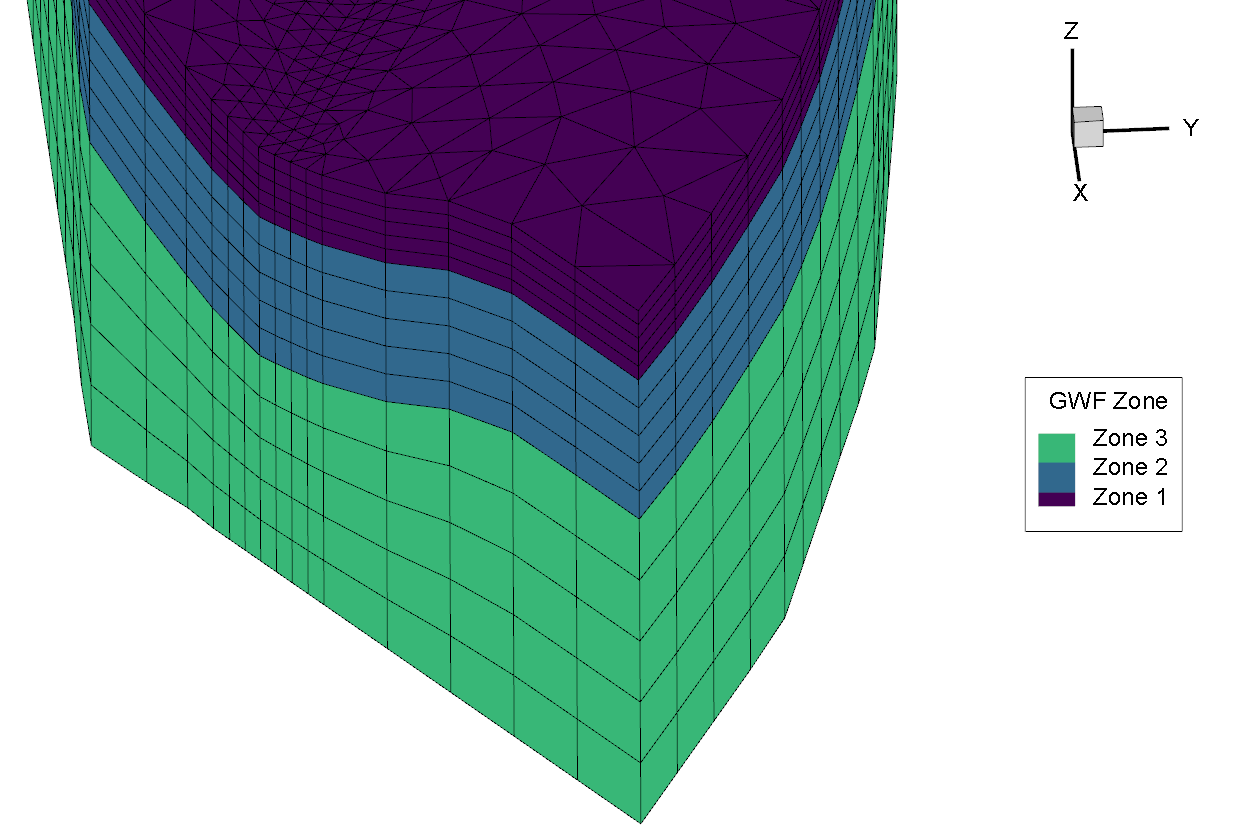
\includegraphics[width=.86\textwidth]{3_10_GWFZones}

Some key features to note are:
\begin{itemize}
    \item There are 3 zones, corresponding to the layers 1 to 3.
    \item 'Zone 1', coloured dark blue, corresponds to layer 1.  Recall that the \mfus\ mesh is generated from the top down, so layer 1 is at the top of the model domain.
    \item Each layer is composed of multiple \mf\ layers, which are each one cell thick.
\end{itemize}

The following section from the input file shows how material properties were assigned for the 3-layer case:
\begin{verbatim}
    gwf materials database
    GWF.csv

    active domain
    gwf

        clear chosen zones
        choose zone number
        1
        choose zone number
        2
        choose zone number
        3

        clear chosen cells
        choose cells by chosen zones

        chosen cells use gwf material number
        5
\end{verbatim}

The following section from the \texttt{eco} file shows zone selection output for the 3-layer case:
\begin{verbatim}
    clear chosen zones
    	GWF Zones chosen:          0

    choose zone number
    	Adding zone number:        1
    	GWF zone numbers currently chosen:
    	    1

    choose zone number
    	Adding zone number:        2
    	GWF zone numbers currently chosen:
    	    1
    	    2

    choose zone number
    	Adding zone number:        3
    	GWF zone numbers currently chosen:
    	    1
    	    2
    	    3

    clear chosen cells
    	GWF Cells chosen:          0

    choose cells by chosen zones
    	GWF Cells chosen:      39765
\end{verbatim}

Some key features to note are:
\begin{itemize}
    \item As we choose zone numbers, the list of currently chosen zones grows accordingly.
    \item The final number of \gwf\ cells chosen is equal to the total number of cells in the domain, since we had selected all 3 layers prior to converting the  zone selection to a cell selection.
\end{itemize}
Since we are assigning uniform properties to the entire model domain, this example could be simplified by simply choosing all cells then assigning properties.  However, if you wanted to assign different material properties to each zone, you can easily do so by modifying the example to assign properties to one zone at a time, being careful to clear the zone and cell selections for each layer.

In some cases, we may want to assign material properties to selected subregions of the model domain.  In such situations, we first select a subset of cells, then assign them a unique zone number using the instruction:

\ins{new zone}
    {Increments the total number of zones in the currently active domain by 1 and assigns that as the zone number of each selected cell.
     }

Below is an example\footnote{See example \texttt{7\_SuperSlab}} in which a \gwf\ model domain which initially had a single zone called {\sf Soil} has had two new zones added called {\sf Slab1} and {\sf Slab2}:

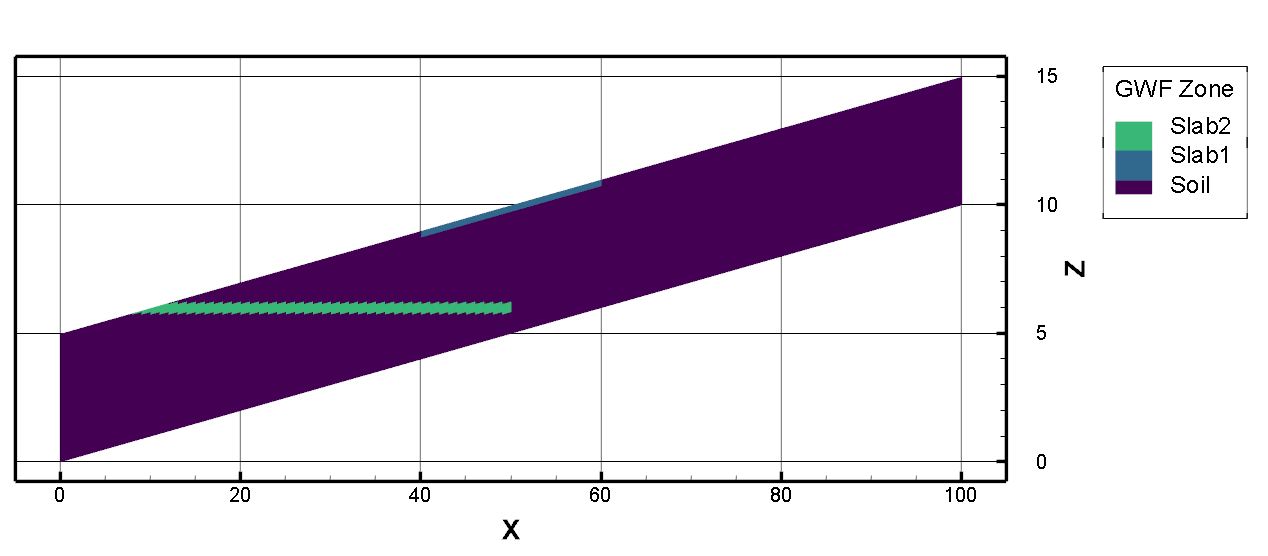
\includegraphics[width=\textwidth]{3_10b_NewZones}

In this example, we introduce the following instruction for selecting arbitrary ranges of cells:

 \ins{choose cells by xyz layer range}
    {
    \squish
    \begin{enumerate}
    \item \rnum{xfrom} [$L$], \rnum{xto}[$L$]  $x$ coordinate range.
    \item \rnum{yfrom} [$L$], \rnum{yto}[$L$]  $y$ coordinate range.
    \item \rnum{zfrom} [$L$], \rnum{zto}[$L$]  $z$ coordinate range.
    \item \inum{LayerFrom}, \inum{LayerTo}  Layer range.
    \end{enumerate}
    Cells whose centroid falls within the given $x$, $y$, $z$ and layer ranges are selected.
    }

\pagebreak
The model zones were defined using these instructions:
\begin{verbatim}
    active domain
    gwf

        choose all cells

        chosen cells use gwf material number
        11

        clear chosen zones
        clear chosen cells
        choose cells by xyz layer range
        40.0  60.0
        -1e30 1e30
        -1e30 1e30
        1   5

        new zone

        choose zone number
        2

        chosen cells use gwf material number
        12

        clear chosen zones
        clear chosen cells
        choose cells by xyz layer range
        8.0  50.0
        -1e30 1e30
        5.8 6.2
        0 1000

        new zone

        choose zone number
        3

        chosen cells use gwf material number
        13
\end{verbatim}


Some key features to note are:
\begin{itemize}
    \item The model has only one zone initially, which is first assigned properties of material 11 (Soil) after choosing all cells in the model domain.
    \item Cells in the range from $x$=40 to $x$=60 and from layers 1 to 5 (inclusive) are chosen and assigned properties of material 12 (Slab1).  Specifying a range between -1e30 and 1e30 means that no restrictions will be applied based on the $y$ and $z$ cell coordinates. Recall that the \mfus\ mesh is generated from the top down, so layers 1 to 5 are the top 5 layers of the model domain.
    \item The first {\sf new zone} instruction increments the total number of zones from 1 to 2 and assigns zone number 2 to the chosen cells.
    \item Cells in the range from $x$=8 to $x$=50 and from $z$=5.8 to $z$=6.2 are chosen and assigned properties of material 13 (Slab2).  Specifying a range between -1e30 and 1e30 for means that no restrictions will be applied based on the $y$ cell coordinates, while a range of 0 to 1000 means that no layer restrictions are being applied.
    \item Because of the sloping nature of the mesh layers, the cells chosen for zone 3 (Slab2) are depicted by \tecplot\ as a 'jagged' boundary, as shown here:

        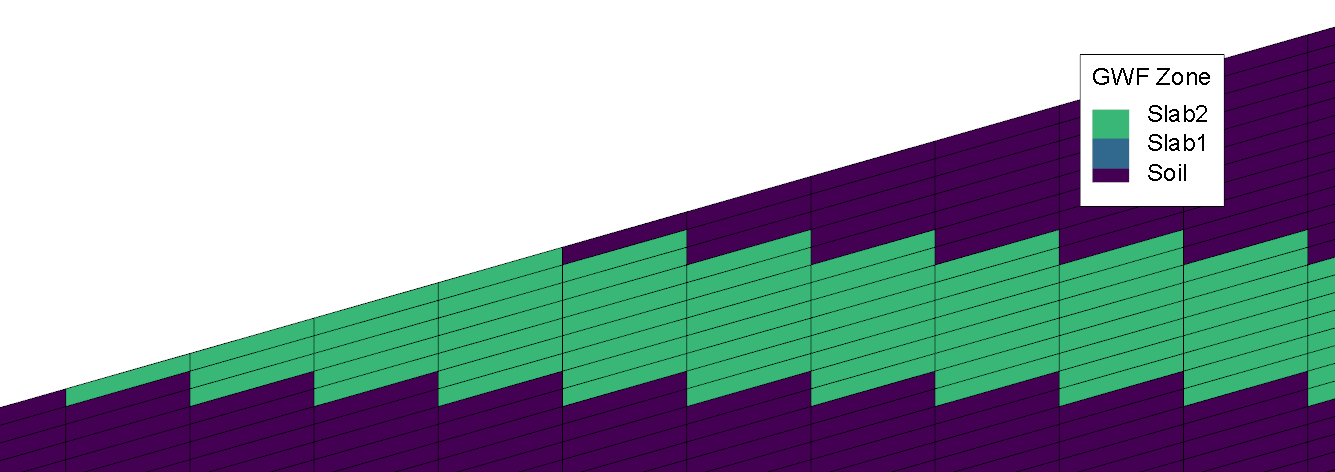
\includegraphics[width=\textwidth]{3_10c_NewZonesJagged}

    \item The second {\sf new zone} instruction increments the total number of zones from 2 to 3 and assigns zone number 3 to the chosen cells.
    \item In this example, zone and cell selections are cleared before defining new zones and assigning material properties, but note that multiple cell selections can be made without clearing to define more complex zones.
\end{itemize}

\subsubsection{Initial Conditions}  \index{\gwf\ Domain ! initial condition ! initial (starting) head}
An initial (or starting) head should be assigned to each cell in the \gwf\ domain.  This could be an initial guess at the beginning of a transient stress period or a set of hydraulic heads from a previous run.

To assign a uniform hydraulic head to the \gwf\ model domain, you must first make a cell selection as described on page~\pageref{page:cellSelect}, then use this instruction:

\ins{gwf initial head}
    {
        \squish
        \begin{enumerate}
        \item \rnum{IHead} [$L$]  Initial (or starting) hydraulic head.
        \end{enumerate}
          An initial hydraulic head  of \rnum{IHead} is assigned to the chosen cells.
    }

As a reminder, \mut\ will echo the assumed units to the screen and \texttt{o.eco} file:
\begin{verbatim}
    gwf initial head
    	Assigning all chosen GWF cells starting heads of     2.7800         METERS

\end{verbatim}


To assign a linearly varying head that is a function of $z$ (i.e.\ depth or elevation), use this instruction:
\ins{gwf initial head function of z}
    {
    \squish
    \begin{enumerate}
    \item \rnum{z(1)} [$L$], \rnum{Head(1)} [$L$]  First $z, head$ pair.
    \item \rnum{z(2)} [$L$], \rnum{Head(2)} [$L$]  Second $z, head$ pair.
    \item \textbf{...}\\
     \hspace*{-.27in}\rule{0.in}{.24in} n. \rnum{z(n)} [$L$], \rnum{Head(n)}  [$L$]  nth $z, head$  pair.
    \end{enumerate}

     An initial head is calculated for each chosen cell, based on it's $z$-coordinate location, by interpolating a head from the given list of  $z, head$ pairs.

    An end instruction is required to stop the subtask e.g.:

    {\Large \sf end gwf initial head function of z}
    }

This is commonly used to generate an initial head for a simple column model\footnote{The example \texttt{1\_VSF\_Column} uses the \texttt{gwf initial head function of z} instruction to define the initial head of the model domain.} as shown here:
\begin{verbatim}
    gwf initial head function of z
    !  z    head
      0.0  -100.0
    100.0     0.0
\end{verbatim}
\pagebreak
Some key features of this example are:
\begin{itemize}
  \item The two given $z,head$ pairs define an initial head  that varies from $head=-100.0$ at $z=0$ to $head=0.0$ at $z=100.0$.  You may supply as many pairs as needed to define the initial head.
  \item $z$-coordinates must increase continuously from the top of the list to the bottom.
  \item the $z$-range of the supplied pairs should cover the entire $z$-range of the model domain.
  \item For each node in the model domain  mesh, the $z$ coordinate is used to interpolate an initial head (i.e. $head$ value) using the appropriate $z, head$ pair.
\end{itemize}

\subsubsection{Boundary Conditions}  \index{\gwf\ Domain ! boundary conditions}
To assign boundary conditions  to the \gwf\ model domain, you must first make a cell selection as described on page~\pageref{page:cellSelect}.

A constant head boundary condition fixes the head at a \gwf\ cell at a given value, allowing water to flow into or out of the \gwf\ model domain depending on surrounding conditions.    To assign a uniform constant head to the \gwf\ model domain use this instruction:

\ins{gwf constant head}
    {
        \squish
        \begin{enumerate}
        \item \rnum{CHead} [$L$]   Constant hydraulic head.
        \end{enumerate}
          An constant hydraulic head  of \rnum{CHead} is assigned to the chosen cells.
    }

A drain boundary condition allows water to flow out of the \gwf\ model domain if the hydraulic head of the cell is higher than the drain elevation.   To add a drain to the \gwf\ model domain use this instruction:

\ins{gwf drain}
    {
        \squish
        \begin{enumerate}
        \item \rnum{DrainK}  [$L$ $T^{-1}$]  Drain conductance.
        \end{enumerate}
          A drain conductance of \rnum{DrainK} is assigned to the chosen cells.  The top elevation of the cell is assigned automatically as the drain elevation
    }

%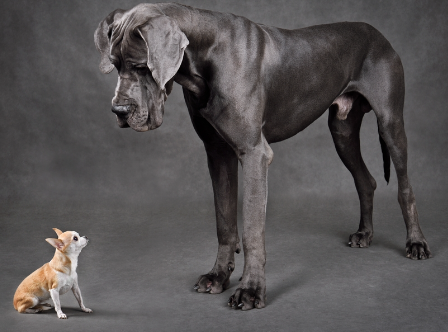
\includegraphics[width=.15\textwidth]{ModelDevelopment} \textit{Should we add an instruction where the drain elevation is specified?  }

A recharge boundary condition forces  water to flow in to the \gwf\ model domain at a specified rate.   To add recharge  to the \gwf\ model domain use this instruction:

\ins{gwf recharge}
    {
        \squish
        \begin{enumerate}
            \item \rnum{RechRate} [$L$ $T^{-1}$]  Recharge rate.
            \item \inum{RechOpt}  Recharge option.
        \end{enumerate}
        A recharge rate of \rnum{RechRate} is assigned to the chosen cells.

        The recharge option \inum{RechOpt} is used to define where the recharge  is to be applied and can have one of the following values:
        \begin{enumerate}
            \item To top layer
            \item To one specified node in each vertical column
            \item To highest active node in each vertical column
            \item To the swf domain on top of each vertical column
        \end{enumerate}
        \squish
    }


A well boundary condition forces  water to flow in or out of the \gwf\ model domain at a specified rate.   To add a well  to the \gwf\ model domain use this instruction:

\ins{gwf well}
    {
        \squish
        \begin{enumerate}
            \item \rnum{PumpRate} [$L^{3}$ $T^{-1}$]  Pumping rate.
        \end{enumerate}
        A pumping  rate of \rnum{PumpRate} is assigned to the chosen cells. Positive pumping rates add water to the domain, negative pumping rates remove water from the domain.
    }



%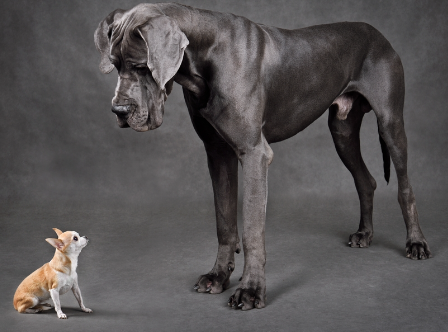
\includegraphics[width=.15\textwidth]{ModelDevelopment} \textit{Should we have an example of pumping with an assigned nodal flux?  Should it be from a CLN?  Is there a boundary condition that assures the head will not be drawn down below the pumping node elevation?}





